\section{Vectors in n dimensional space}
A n-dimensional Euclidean space $\mathbb{R}^n$ is a natural extension of 2 dimensional Euclidean place and 3 dimensional Euclidean space. An n-dimensional vector is represented as a row vector or column vector by $\mathbf{a} = (a_1, \dots, a_n)$ or 
$$
\mathbf{a} = \begin{pmatrix} a_1 \\ \dots \\ a_n \end{pmatrix}
$$

We use bold face lowercase letter to represent vector and normal face lowercase letter to represent the scalar.

The addition and scalar multiplication for a vector $\mathbf{a}$ can be summarized as $\lambda \mathbf{a} + \mathbf{b}$ where $\lambda$ is a scalar and $\mathbf{b}$ is another n-dimensional vector.

To write it in specific form, we have $\lambda \mathbf{a} + \mathbf{b} = (\lambda a_1 + b_1, \dots, \lambda a_n + b_n)$.

The inner product of two n-dimensional vector is defined as $\b{a} \cdot \b{b} = \sum_{i=1}^n a_i b_i$. It is an extension of inner product of two vectors in 2 or 3 dimensional Euclidean space. If $\b{a} \cdot \b{b} = 0 $, we call $\b{a}$ is orthogonal to $\b{b}$.

The 2 norm for a vector $\b{a}$ is defined as $\norm{\b{a}}_2 = \sqrt{\b{a}\cdot \b{a}}$.

There are some notation simplification in other places. For example, 2 norm is the default norm for a vector, we can write it simply as $\norm{\b{a}}$. If the summation index range is obvious, we can write $\sum_{i}$ instead of $\sum_{i=1}^n$.

\section{Basis in n-dimensional space}
Given $r$ vectors $\b{a}_1 \dots, \b{a}_r$ in n-dimensional space, we say they are independent if $ \sum_{i=1}^r c_i \b{a}_i = 0 \Rightarrow c_i = \b{0} \textrm{ for } i=1,\dots r$.
Otherwise, we say there are dependent vectors.
\begin{example}
$\b{a}_1 = (1, -1)$ and $\b{a}_2 = (2, 1)$. Then $c_1 \b{a}_1 + c_2 \b{a}_2 = (c_1 + 2 c_2, -c_1 + c_2 ) = (0,0) \Rightarrow c_1 = 0, c_2 = 0$. Therefore, $\b{a}_1$ and $\b{a}_2$ are independent. Let $\b{a}_3 = (1, -3)$, we have $-\frac{7}{3} \b{a}_1 + \frac{2}{3} \b{a}_2 + \b{a}_3 = (0,0)$. Therefore, $\b{a}_1, \b{a}_2, \b{a}_3$ are dependent vectors.
\end{example}
A fundamental theorem states that for a n dimensional space, there exists $n$ vectors which are independent; and for arbitrary $n+1$ vectors, they are dependent.

Suppose $\b{e}_1, \dots, \b{e}_n$ are n independent vectors. For another vector $\b{a}$, since
$\b{e}_1, \dots, \b{e}_n, \b{a}$ are dependent vectors, we can show that there exists unique $c_i$ such that
$\b{a} = \sum_{i=1}^n c_i \b{e}_i$. We call $\b{e}_i, i=1,\dots n$ a basis of $\mathbb{R}^n$ and $(c_1, \dots, c_n)$ is the coordinate of the vector $\b{a}$.

If $\b{e}_1, \dots, \b{e}_n$ are mutually orthogonal and $\b{e}_i \neq \b{0}$, they form an orthogonal basis of $\mathbb{R}^n$. Indeed,  for $\sum_{i=1}^n c_i \b{e}_i = \b{0}$, applying dot product with $\b{e}_j$ on both side of the equation, we can get $ c_j \norm{\b{e}_j}_2^2 = 0 $. Then $c_j = 0$. and $\b{e}_1, \dots, \b{e}_n$ are mutually independent. The coordinate of $\b{a}$ with respect to an orthogonal basis is easy to compute. $\b{a} = \sum_{i=1}^n c_i \b{e}_i \Rightarrow c_i = \frac{\b{a}\cdot \b{e}_i}{\b{e}_i\cdot \b{e}_i}$
\begin{figure}[!ht]
	\centering
	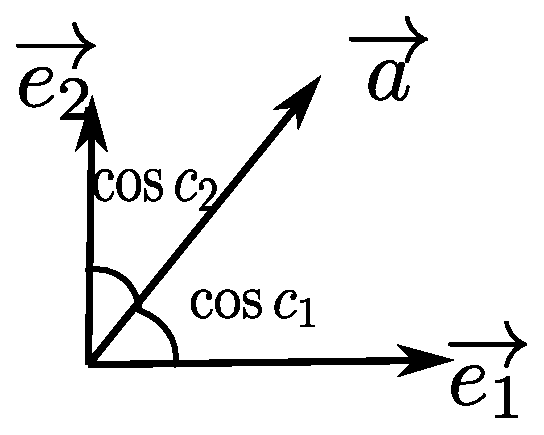
\includegraphics[width=5cm]{orthogonal_basis.eps}
	\caption{A illustration of orthogonal basis in $\mathbb{R}^2$}
\end{figure}

\section{Matrix and its property}
In the above section, we have $\b{a} = \sum_{i=1}^m c_i \b{e}_i$ where $m=n$. In this section, we are not restricted to the case $m=n$. Let $\b{e}_i = (e_i^1, \dots, e_i^n)$. We can write the expression in the following form:
\begin{equation}
	\begin{pmatrix} a_1 \\ a_2 \\ \dots \\ a_n \end{pmatrix}
	 = \begin{pmatrix} e^1_1 & e^1_2 & \dots & e^1_m \\ e^2_1 & e^2_2 & \dots & e^2_m \\ 
	 	\vdots & \vdots & \dots & \vdots \\
	 	 e^n_1 & e^n_2 & \dots & e^n_m \end{pmatrix} \begin{pmatrix} c_1 \\ c_2 \\ \dots \\ c_m \end{pmatrix}
\end{equation}
The linear transformation from vector $\b{c}$ to $\b{a}$ is represented by the matrix $\b{E}$, which has $n$ rows, $m$ columns and $\b{E}_{ij} = e^i_j$.
Matrix $\b{E}$ transforms a $m$ dimensional vector $\b{c}$ to $n$ dimensional vector $\b{a}$ and 
we have the following sufficient notation for the transformation:
\begin{equation}
\b{a} = \b{E}\, \b{c}
\end{equation}
The dimension for a matrix $\b{E}$ is characterized by two numbers $(m,n)$. We call $\b{E}$ is a $m\times n$ matrix.

The addition and scalar multiplication for a matrix $\b{E}$ can be defined similarly. Let $\b{C} = \lambda \b{A} + \b{B}$ where $\b{A}, \b{B}$ have the same dimension, then $\b{C}_{ij} = \lambda \b{A}_{ij} + \b{B}_{ij}$.

Suppose we have two matrices $\b{A}$ and $\b{B}$.  $A$ is with dimension $(m,n)$ and $\b{B}$ is with dimension $(n,r)$. We can multiply matrix $\b{A}$ by $\b{B}$ and get the resulting matrix $\b{C}$ with dimension $(m, r)$. The multiplication rule is $\b{C}_{ij} = \sum_{k=1}^n \b{A}_{ik}\b{B}_{kj}$

\begin{exercise}
Suppose $\b{A}, \b{B}, \b{C}$ are $m\times n, n\times r, r \times t$ matrices respectively.	Show that $\b{A}(\b{B}\b{C}) = (\b{A}\b{B})\b{C}$.
\end{exercise}
\section{Linear Equation System}